\documentclass[12pt]{article}
\usepackage{float}
\usepackage{graphicx} % Required for inserting images
\usepackage{fontspec}
\usepackage{apacite}
\setmainfont{Times New Roman}
\usepackage[letterpaper,top=2cm,bottom=2cm,left=2cm,right=2cm,marginparwidth=1.5cm]{geometry}

\title{01 - Reflection on own knowledge and skills on human and social aspects of cybersecurity}
\author{Truong Khang Tobias Nguyen}
\date{}

\begin{document}

\maketitle

\section{Figure} 

\begin{figure}[H]
\centering
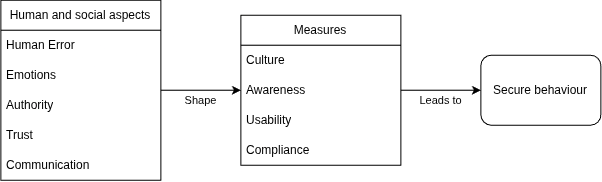
\includegraphics[width=0.75\linewidth]{figure.png}
\caption{Figure explaining my understanding of human and social aspects of cybersecurity.}
\end{figure}

\section{Explaination}

This figure explains my understanding of human social aspects of cybersecurity. On the left, I have noted the human and social factors that come to my mind in cybersecurity. Nowadays, cybersecurity incidents often involve social engineering, e.g. tricking a human to click on a phishing link or into giving credentials, etc. rather than technical faults \cite{siddiqi2022study}. I can think of five attributes that are especially vulnerable which are the following:
\begin{itemize}
\item \textbf{Human errors} as sometimes attackers don’t need to proactively attack a system but can wait until the system's users make mistakes, like clicking on a phishing link or input information somewehere they aren't supposed to. 
\item \textbf{Emotions} as attackers can exploit certain emotional attributes such as helpfulness, fear or urgency which can in suppress our ability to think critically.
\item \textbf{Authority} as attackers can pretend to be a figure of authority like police, politicans or managers to force us into actions we normally wouldn't do for others. This attribute is closely related to \textbf{emotions} as they pretend to be someone in power to give us a sense of fear or urgency.
\item \textbf{Trust} as our trust can be exploited by attackers. If we take the \textbf{authority} attribute as an example, if an attacker pretends to be a person in power, we would think of them as trustworthy and thus, think less critical when we help them.
\item \textbf{Communication} as poor communication between people can also be exploited. Either by malicious actors or even by organizations. For example, after an incident, the fear of retaliation could potentially lead humans to not report them, resulting in incidents going unnoticed.
\end{itemize}
As these attributes can be exploited, they especially have to be considered when developing security measures and thus, shape them. The middle box consists of four measures that stem from the human and social aspects explained and are:
\begin{itemize}
\item \textbf{Culture:} Building a culture where people feel safe and don't get punished for making mistakes or reporting incidents.
\item \textbf{Awareness:} People should know what type of attacks exists and how they can avoid, reduce or mitigate them.
\item \textbf{Usability:} Security tools should integrate well into work or actions of people, otherwise they may not use them.
\item \textbf{Compliance:} People should know what they can or cannot do and also should be aware of the consequences if these rules are disregarded. 
\end{itemize}
I believe that these measures can help to reduce attacks that them from the aforementioned human and social aspects and that they will lead to secure behaviour in people, whether in a work environment, in private, social media, etc. 

\section{Reflections}

As I have a technical background, I didn't have any coursework or experiences regarding human and social aspects in any capacity and therefore, I am unfamiliar with this topic.
I am aware that the nature of cyberattacks isn't purely technical and aren't just attacks on technical systems, but also an attack on human behaviour \cite{indrajit2017social}. 
\newline
As humans become targets in cyberattacks, I believe that it is necessary that we development measures that protect the human and social attributes that can be exploited and the figure in the first sections shows which aspects I believe need to be considered and what measures can be taken to protect them.
\newline
As someone coming from a technical background, I want to learn which human and social aspects are vulnerable to cyberattacks, why they are vulnerable and how they can be exploited. I am especially interested in learning how to develop suitable security measures based on these aspects and how to actually implement them in a business setting and if the course goes into it, I would also love to learn on how to get from these aspects and measures and define security specifications when developing systems, services and applications.
\newline
In order to achieve this, I plan to not only just do the mandatory readings, but also some of the optional readings as well and look for relevant industry articles when it comes down to the more practical topics like implementing said aspects to a business setting.

\bibliographystyle{apacite}
\bibliography{references}

\end{document}